% FIXME -- polish related works

% \section{Research Area Introduction}
\section{Research Area Introduction}

\label{sec:Research area introduction}

%FIXME useless next lines
In this section, the details of various approaches and the \ac{sota} in 3D \ac{hpe} are presented along with some works in the sibling task of hand pose estimation. The aim of this section is to give an overview of how the problem of 3D \ac{hpe} is tackled in the literature.

\subsection{Pose from images}

Numerous works try to estimate 3D human poses from 2D \ac{rgb} images or 2D joint confidence heatmaps \cite{CameraDistanceAware, poselifter, DistillNRSfM, occlusionVideo, ordinalranking}. Most of these methods follow a cascading approach, where an explicit intermediate representation of 2D pose or 2D heatmaps is used.

For example, \cite{CameraDistanceAware} proposes a general framework with 3 networks. Human detection Network, RootNet, PoseNet. Where the human
detection network predicts the region the human is in an image. The RootNet localizes the human's root in the global 3D world. And, the PoseNet
predicts the 3D pose of a single person relative to the root. Where the root is a fixed reference point of the human body say, pelvis.

The advantage of such top-down frameworks is to divide the task of RGB to 3D into smaller, well-studied sub-tasks. This makes scaling single-person
pose estimation algorithms for multi-person pose estimation easy, as the majority of the data available mostly consists of a single person per
frame. In addition to it, this approach provides the opportunity to improve certain modules without affecting or having to re-train the other modules
of the system.

\subsection{Pose Lifting}

In contrast to the estimating pose from an image, Pose Lifting works such
as \cite{poselifter,  amazon1, repnet, c3dpo, unsupervisedAdversarial},
focus on estimating 3D poses from 2D poses alone. Assuming 2D poses from
the \ac{sota} methods in 2D \ac{hpe}. These methods include simple linear
models as first described in \cite{MartinezHRL17} with a series of fully
connected linear layers, and sometimes batch normalization, dropout and,
residual connections to regress 3D pose effectively.

\ac{nrsfm} is another promising lifting method that also leverages images
along with 2D annotations. \ac{nrsfm} deals with the problem of
reconstructing 3D shape (pose/point cloud) and cameras of each projection
from a sequence of images with corresponding 2D orthogonal projections (2D
keypoints). This approach has been widely used in facial keypoint detection
and \cite{deepNRSFM} introduces deep learning variant for the same. Instead
of predicting the 3D coordinates of each keypoint/joint of the 3D pose,
\cite{DistillNRSfM, c3dpo, deepNRSFM, nrsfm++} predicts the 3D shape and
camera pose from 2D pose using this method.

The Pose Lifting approach facilitates to leverage the already well
established 2D \ac{hpe} models that are trained on enormous and diverse
labeled data. Thus demanding lesser training data for 3D pose estimation
than it would need when learning from images. Since these networks do not
have large convolution layers they are less computationally inexpensive for
both training and inference on edge computing units. Moreover, the 2D and
3D pose data usually can be entirely loaded onto the GPU further
accelerating the training procedure. Thus addressing the critical problem
that hinders scalability of 3D \ac{hpe} models and also helps to develop
better modular systems by combining the best of Pose Lifting networks with
the best of 2D \ac{hpe}. However, due to the inherent ambiguity in lifting
pose to 3D and as the images are not captured with orthogonal cameras,
reprojection of 3D pose will vary from the ground truth, it is challenging
to match the performance of models trained on 3D ground truth.

\subsection{Non-Supervised Learning}

The standard way to train 3D/2D \ac{hpe} is by minimizing the distance
between the predicted 3D/2D pose and its corresponding ground truth. The
area of 2D \ac{hpe} is well established and matured with reliable systems
deployed in the real world. This was made possible with the high volume of
images from diverse settings and the reasonable ease of manual labeling of
2D poses. On the other hand, labeling 3D pose manually is not practical.
Though single-person datasets such as Human3.6M \cite{H3.6}, Human Eva \cite
{HumanEva} and, multi-person datasets such as CMU Panoptic \cite
{cmuPanoptic} provide 3D pose ground truth. They are obtained using \ac
{mocap} systems which are only limited to indoors or cannot be directly
adapted to outdoor environments where the majority of the use cases exist
fig[\ref{fig:h36_mocap}]. It is also worth mentioning JTA(Joint Track Auto)
dataset \cite{JTA} that is made using the GTA(Grand Theft Auto) game engine
which is technically scalable with its own limitations. But datasets from
simulations come with the difficulty of domain adaptation to be
transferable to the real world.

\begin{figure}[!h]

    \centering

    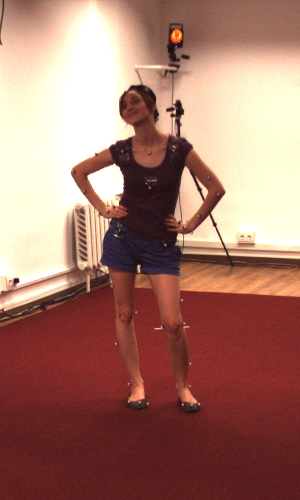
\includegraphics[width=30mm]{figures/h36_mocap.png}

    \caption{Image from Human3.6 Dataset \cite{H3.6} of subject wearing \ac
        {mocap} markers}

    \label{fig:h36_mocap}

\end{figure}

To overcome this bottleneck, \cite{unsupervisedAdversarial} proposes
unsupervised training of a generative adversarial network by projecting the
predicted 3D pose back to 2D and minimizing its distance with the input 2D
pose. And further training a discriminator to distinguish the real 2D pose
from the projected poses. Thus removing the need for any explicit 3D
annotations besides 2D poses that are either manually labeled or obtained
using 2D \ac{hpe} models. RepNet \cite{repnet} trains an adversarial
network without 2D-3D correspondences in a weakly supervised manner.
Moreover, it also does not require camera parameters to project the 3D pose
but learns to predict them. Thus enabling better generalization to more
diverse data with unknown cameras and poses.

To test the maximum capability of Pose Lifting networks, \cite{amazon1}
proposes a combination of unsupervised and adversarial learning that mainly
leverages the property of \textit{plane-invariance}. It is the property
that 2D projections of a 3D pose from different camera viewpoints, when
lifted should produce identical and the original 3D pose. In this method,
the predicted 3D pose is rotated in random angles and is reprojected to 2D
in a different \ac{pov}. A discriminator is then used to evaluate if this
new 2D pose is in the possible pose distribution which is learned from 2D
pose datasets alone. These steps are redone in reverse order to obtain the
original 2D input. This cycle provides three intermediate representations
of the single 2D input that the models learn from. Additionally, this
approach exploits the temporal consistency in the datasets as well as
integrates a domain adaptation network to learn from different datasets and
distributions to achieve comparable results to that of the methods that
require more supervision.

\subsection{Multimodal Representation Learning}

\label{section:multimodal_representation_learning}

Another interesting approach is training \ac{vae}s using multiple
modalities like images, poses, depth maps \cite{CrossingNets, crossmodal,
    MMVAE,HandDisentangled}. \ac{mvae}s learn representation from different
modalities in the same latent space. True multimodal learning needs to
fulfill 4 criteria as follows: i) \textit{Latent Factorization} - Implicit
factorization of latent space into private, shared subspaces based on
modality as illustrated in the figure[\ref{fig:criteria}]. ii) \textit
{Coherent Joint Generation} - Coherence in generations of different
modalities from the same latent value with respect to the shared aspects of
the latent. iii) \textit{Coherent Cross Generation} - Generation of one
modality conditioned on data from different modality while preserving the
similarity between them. iv) \textit{Synergy} Enhancement in generation
quality of one modality as a result of learning representations of
different modalities.

\begin{figure}[!h]

    \centering

    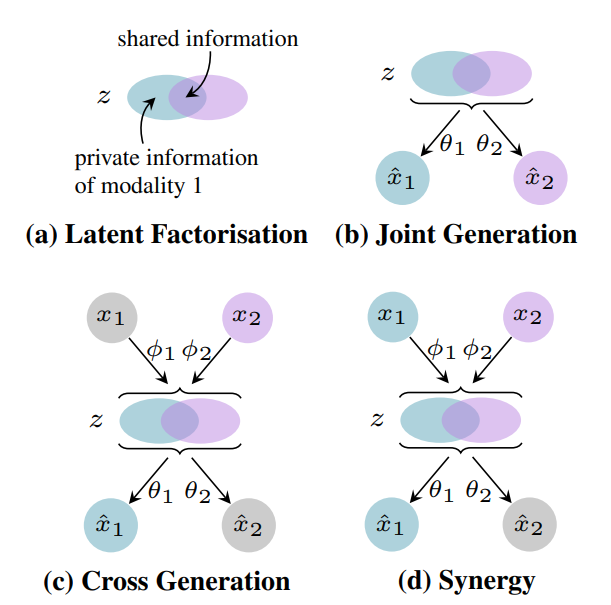
\includegraphics[scale=0.4]{figures/criteria.png}

    \caption{Criteria for Multimodal Generation \cite{MMVAE}}

    \label{fig:criteria}

\end{figure}

\ac{mmvae} proposed by \cite{MMVAE} fulfills all 4 of the above-mentioned
criteria learning representations of image and text data, while other
approaches focus on leveraging specific advantages of multimodal learning.
Consider the cross-modal learning for 3D Hand Pose Estimation proposed by
\cite{crossmodal}. It involves training an encoder-decoder pair to learn
image representation, and another such pair to learn 3D hand pose
representations in the same latent space. This training procedure focuses
on cross-generation and synergy. That is, using the shared latent space of
the image and pose representations, the \ac{rgb} image encoder combined
with the pose decoder can generate 3D poses and vice versa while preserving
the commonality between the conditioned and the generated data. With this
approach, it is possible to train a \ac{vae} for 3D \ac{hpe} from \ac{rgb}
images without explicit intermediate stages like the earlier mentioned
cascading approaches. Making it more efficient and fast for both training
and inference without compromising the modularity offered by cascading
approaches.

%TODO add exemplar methods

\section{Related Work - A closer look}
\label{section:Related Work}

In this section, works that are directly related to the thesis are discussed in more detail. Some are the best examples of their kind and have already been discussed thoroughly. The basic idea of the thesis is to learn 3D \ac{hpe} just from 2D pose data without using 3D ground truth in any shape or form. Thus developing a method that can exploit the huge amounts of 2D pose data that can be generated using state of the art 2D pose networks on diverse images from the real world. The following approaches uses weakly supervised or unsupervised approaches to accomplish the same. These serve as the inspiration for many of the choices taken in this thesis and also help understand the possibilities of reducing the need for explicit 3D supervision.

% FIXME better cite instead of just using numbers
To the best of knowledge acquired during the period of the thesis, \cite{can3dpose, amazon1, unsupervisedAdversarial, c3dpo} are the main approaches that do not use 3D supervision in any way. While \cite{repnet, weaklymultiple} are among the main appraoches the use 3D supervision to train the discriminator alone. The approaches that are not mentioned are either the approaches the above mentioned are built up or have been missed during the literature study.

\cite{unsupervisedAdversarial, can3dpose, amazon1} can be viewed as a series of approaches that are built on one another in the same order. They take 2D poses as the input and learn to predict the depth offset for each joint to reconstruct 3D. Out of the three Ching et al. \cite{amazon1}, using the plane invariance, geometric self-supervision and adversarial learning as discussed in \ref{sec:Research area introduction}, achieves the \ac{sota} results compared to fully supervised methods and also present ways to use domain adaptation network, temporal consistancy to further integrate more datasets and improve the performance. Thus directly address the hudles of scaling the 3D \ac{hpe} network to the real world. However, they also ackwoldge the fact that most of the prediction made by \ac{sota} 2D \ac{hpe} model on real world images had missing joints. Since the proposed approaches only predict the depth of every joint, the error from the 2D input pose is directly propogated to the 3D prediction. More importantly, it is not possible to use most of the data that is generated from 2D pose models. Hence it is very crutial to handle the problem of \textit{\textbf{missing joints}} to truly unlock the potential of unsupervised learning. 

Wandt et al. \cite{repnet} also discused in \ref{sec:Research area introduction} proposes an architecture that learns to predict the whole 3D pose, while also learning the camera parameters that are used to project the predict 3D to 2D. The idea behind the camera network is to learn the view angle given pose to generalize to unknown cameras. The pose network learns to converge the predcited 2D reprojections, while using a \ac{gan} trained on \textit{\textbf{3D ground truth labels}} to supervise the predicted 3D pose. Though there is no direct error propogation from 2D input to 3D, it is important to note the problem of missing joints is not yet addressed. 

However, there another fundemental problem still persists. As mentioned in \ref{sec:background}, 2D-to-3D pose lifting is an ill-posed-inversed problem due to \textit{\textbf{depth ambiguity}} as there are multiple plausible 3D poses that gives the same 2D projection. Addressing this problem, Chen Li et al. \cite{multiplehypo} proposes a varaitional inference model inspired by the architecuture of Wandt et al. \cite{repnet} that takes 2D pose along with a \textit{latent code} to produce 3D pose. The predicted 3D pose varies according to the latent code while maintaining the same 2D reprojection. This varaitional inference of 3D pose addresses both the problems of depth ambiguity and missing joints. 

The above approach has been further improved by Chen Li et al. in \cite{weaklymultiple} to leverage adversarial training using \ac{gan} trained using 3D ground truth. Though there is no direct supervision on 3D pose, 3D data is still required to train this network. It is important to note that in the case where large amount of 3D ground truth poses are available, they can be easily exploited to generate 2D poses of large volume and it is not practical to get 3D poses in the wild to scale the models. In this thesis we try to address all the forementioned problems.
